\documentclass{standalone}
\usepackage{tikz}
\begin{document}
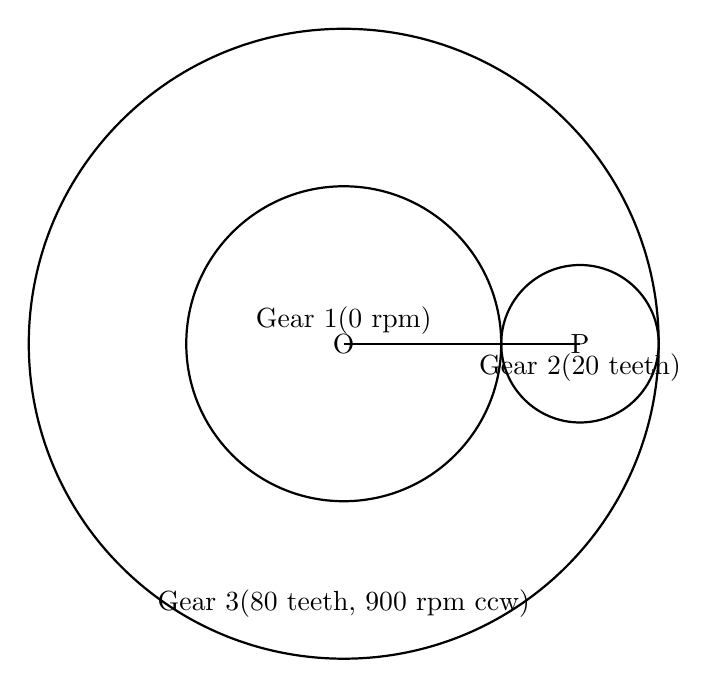
\begin{tikzpicture}
    % Gear 1 (Center circle)
    \draw[thick] (0,0) circle (2cm);
    \node at (0,0) {O};
    \node[above] at (0,0) {Gear 1 \\ (0 rpm)};
    
    % Gear 2 (Smaller circle on the right)
    \draw[thick] (3,0) circle (1cm);
    \node at (3,0) {P};
    \node[below] at (3,0) {Gear 2 \\ (20 teeth)};
    
    % Connecting rod between Gear 1 and Gear 2
    \draw[thick] (0,0) -- (3,0);
    
    % Gear 3 (Outer circle)
    \draw[thick] (0,0) circle (4cm);
    \node[below] at (0,-3) {Gear 3 \\ (80 teeth, 900 rpm ccw)};
    
\end{tikzpicture}
\end{document}
